\section{Dataset Construction}





In this section, we will introduce the construction of CogBench. 
We will introduce image collection, annotation, tasks and the statistics of CogBench.
% Then, we will introduce tasks in CogBench.
% Last, we will show the statistics of CogBench.
% Figure \ref{fig:cogbench} shows an overview of CogBench through an example.
% Ethical considerations of CogBench are discussed in Appendix \ref{sec:ethical}.


\subsection{Image Collection}

\begin{figure}[htbp]

\centering
% \raisebox{30mm}{ % 调整这个值以向上移动图片和caption
%   \parbox{0.98\textwidth}{
    \centering
    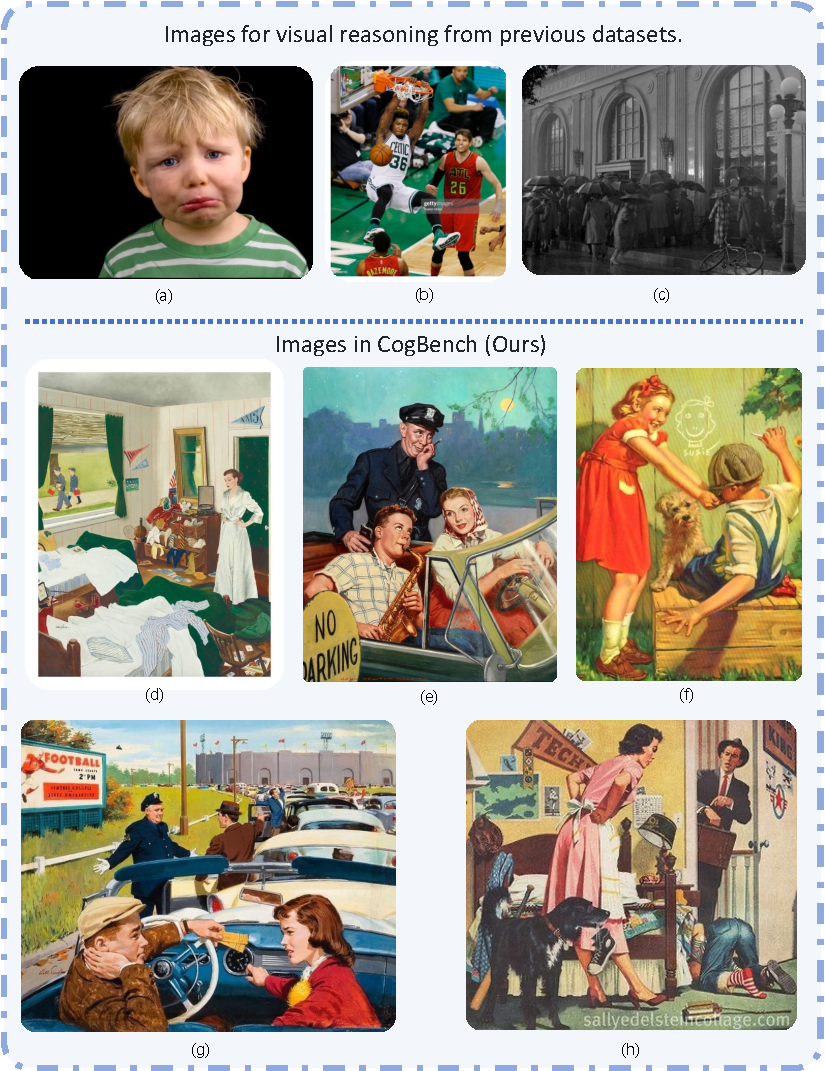
\includegraphics[width=0.4\textwidth]{figs/cog_img_example2.pdf}
    % \vspace{-15pt} 
    \caption{The comparison between our images and those from the previous visual reasoning tasks.
    Compared to our images, image (a) has fewer entities and CoRs, image (b) and (c) have some entities, but fewer CoRs.
    }
    \label{fig:cogbench_example}
    % }
% }

\end{figure}

% One of the most important reasons that Cookie Theft picture description task can be widely used as an effective tool to evaluate human cognitive ability is that the picture is carefully designed. \KZ{This sentence is again useless and
% you are repeating yourself.} 
% Therefore, to align with Cookie Theft, images in CogBench are also carefully collected to meet the requirements of picture design in human oriented picture description task as much as possible. \KZ{You can delete this para.}




Based on previous studies \cite{describe-ctp, tasnim-etal-2022-depac}, we set the following image collection criteria: 
% \MY{can you give names to these rules? short and to the point ones, e.g. Rule1 stroy-telling; Rule 2: High information density; ...}

\begin{itemize}
    \item \textbf{Rule 1: Story-telling} The image depicts an interesting story. For instance, the Cookie Theft picture tells the story of a mother busy washing dishes while two kids takes the opportunity to stand on a stool and sneakily steal cookies.  % Those images simply depict a single event (e.g. a boy is running),  or a scene without a clear story (e.g. a picture of a restaurant) are not considered.
    % \item \textbf{Rule 2}: The image contains one or more subjects (human or animal), engaging in different events.
    % relationships between components
    \item \textbf{Rule 2: Rich Chain-of-Reasonings} Images should display rich Chain-of-Reasonings (\underline{\textbf{CoR}s}) in a scene. 
    % A CoR connects low-level events or conditions in network of causalities. 
     A CoR connects low-level observations in an image to produce a high-level reasoning conclusion or connects the cause and effect of events.
    For example, ``The mother is busy washing dishes. + The boy is standing on the stool behind the mother. + The girl standing by the boy is shushing him. + The boy is fetching cookies from the jar in the cabinet. $\rightarrow$ The boy and girl are stealing cookies.'' is a CoR about high-level event ``stealing cookies''. Note that the story is actually constructed via these CoRs.
    \item \textbf{Rule 3: Restricted Content Complexity} Images should contain rich content but not be overly complex. The number of entities should be sufficient to support a good story while being restricted to emphasize the key points effectively. 
    % limited to avoid being overwhelming.
    % enough to emphasize the key points effectively. 
    % Content Simplicity
    %facilitating description by humans or models. 
    % \KZ{Rich content and simple content seems to be contradictory. Maybe ``appropriate content richness?'' What is appropriate? I think it's enough entities to support a good story. So ultimately it's about stories.}
    % For those pictures with a lot of subjects, even they are rich in content and there might be interesting stories in them, it is difficult for models or even humans to describe them in a short time. Therefore, we do not consider these pictures.
\end{itemize}

% \begin{wrapfigure}{l}{0.5\textwidth}
% \begin{figure}[th]
%   \centering
%   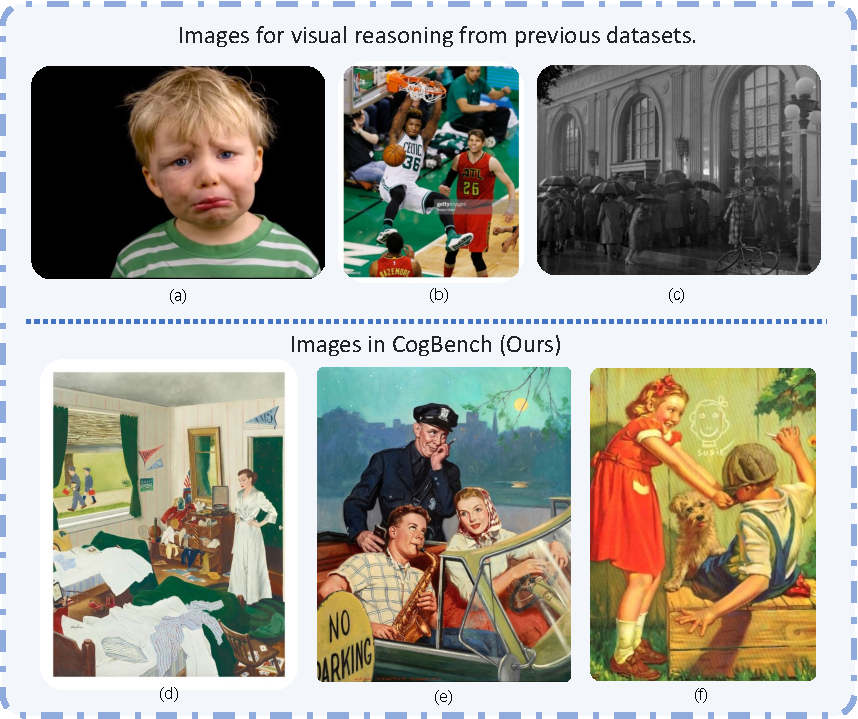
\includegraphics[width=0.45\textwidth]{figs/cog_img_example.pdf}
%   \caption{The comparison between our images and those from the previous visual reasoning tasks.
%   Compared to our images, image (a) has fewer entities and CoRs, image (b) and (c) have some entities, but fewer CoRs.
%   \KZ{This fig wastes space, maybe combine it with another fig in one row.}
%   % \MY{can you add elements contrast here? e.g. previous datsets have entity, but few CoRs. The selected pics are not that contrastive (we are trying to say that exsiting datasets involve simple pictures), picture A and C are quite similar to something can be involved in our dataset, where you can infer a lot of things.}
% }
%   \label{fig:cogbench_example}
% \end{figure}
% \end{wrapfigure}


With the above criteria, 
%we aim to select high-quality images for cognition evaluation of LVLMs. 
% Currently, we have collected 95 images for CogBench. 
we manually collect pictures from Pinterest\footnote{\url{https://www.pinterest.com/}}, 
and the Cookie Theft is also included. % in CogBench.

The image selection criteria above define the characteristics of the Cookie Theft-like images that we proposed.
\figref{fig:cogbench_example} shows the differences between our images and those from other datasets by examples.
% \MY{We should say how many pics were included first, then screened out by which rule, and ended up with xxx. Do we have an annotation-based filtering as well? Like after annotation, some pics are too simple or too difficult then it's excluded at last.}
% \XJ{As the collection cretiria are strict, we do not filter out too many images.}

\subsection{Image Annotation}
\label{sec:annotation}


\begin{figure*}[h]
  \centering
  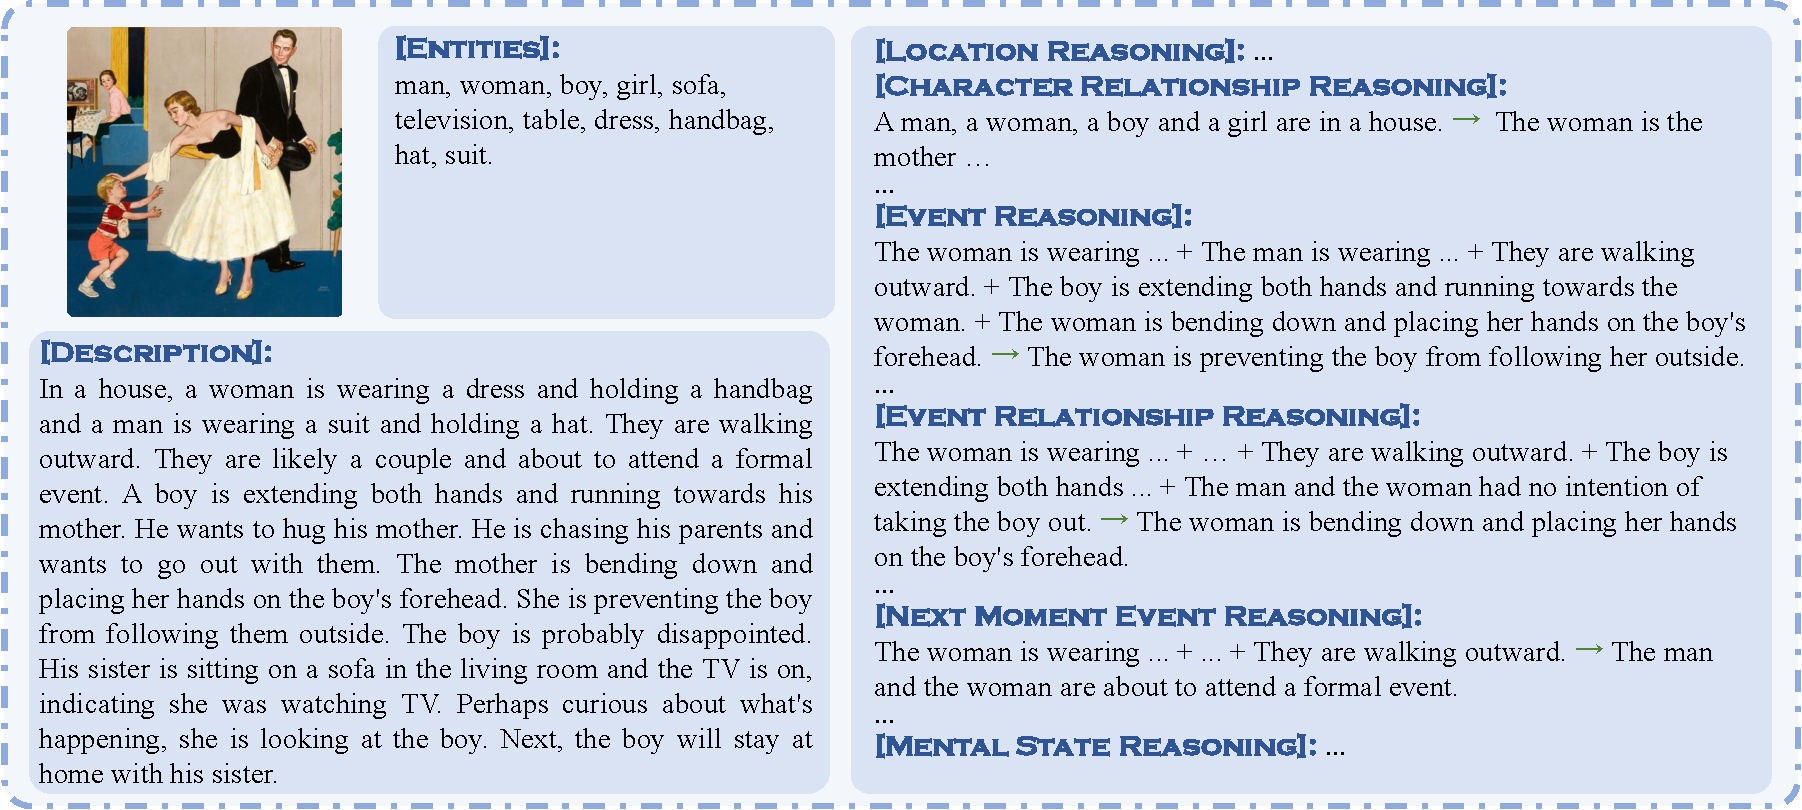
\includegraphics[width=0.95\textwidth]{figs/descrption_task_4.pdf}
  \caption{An example of Description task from CogBench. 
  % \KZ{The fonts are too small.
  % No need to include everything. You can include a complete example in the 
  % appendix.} \MY{separate VQA into another figure, it will simplify this one and make it easier to understand}
  % \XJ{font size increased.}
}
  \label{fig:cogbench}
\end{figure*}


Human annotators, mostly undergraduate or graduate students aged 18-28, are hired to annotate the collected images.
% \footnote{Wages and recruitment process details can be found in Appendix \ref{sec:ethical}.}
% \MY{add cross ref to this}}. 
% The annotators are mostly undergraduate or graduate students with normal cognitive functioning, aged between 18 and 28.
As shown in Figure \ref{fig:cogbench}, the annotation includes three parts: [Entities], [CoRs] and [Description].
By annotating [Entities] and [CoRs], we aim to evaluate the low-level recognition ability and high-level cognitive reasoning ability of models respectively based on description. 
% By annotate , we aim to evaluate the high-level cognitive reasoning ability of models during description. 
% [CoRs] can also be used for generating questions for CogVQA task.
[Description] is annotated as the reference description for the image.
The three parts are annotated in that order. 

% [Entities]
\noindent\textbf{Entity Annotation} We ask annotators to list as many entities in the image as possible and entities
that are difficult to recognize should be omitted. 

\noindent\textbf{CoR Annotation} %Annotators are asked to annotate high-level CoRs in the image. 
In order to evaluate model cognition in a fine-grained manner, the following eight reasoning dimensions are annotated with corresponding CoRs:

\begin{itemize}
  \item \textbf{Special Time Reasoning}: reasoning about the special time of the story in the image, e.g., festivals, seasons etc.
  \item \textbf{Location Reasoning}: reasoning about the location of the story in the image, e.g., near the school etc.
  \item \textbf{Character Reasoning}: reasoning about the character of the subjects in the image, e.g., police officer etc.
  \item \textbf{Character Relationship Reasoning}: reasoning about relationship between characters in the image, e.g., ``the woman is the mother of the kids.''
  \item \textbf{Event Reasoning}: reasoning about high-level events in the current moment and previous moments in the image based on clues in the picture. The difference between high-level and low-level lies in how much semantic information the event contains, e.g., ``stealing cookies'' is a higher-level event compared to ``taking cookies'' as it additionally conveys the semantic of ``taking advantage without permission or knowledge.''
  
  \item \textbf{Event Relationship Reasoning}: reasoning about causal and temporal relationship between different events in the image. For instance, ``the sink is overflowing \textbf{because} the mother left the tap on.'' 
  % These events are usually linked through causal and temporal relations \cite{describe-ctp}. 
  \item \textbf{Next Moment Event Reasoning}: reasoning about the event that will happen in the next moment. For example, ``The police officer will reprimand the boy who violates the rules.''
  \item \textbf{Mental State Reasoning}: reasoning about the mental states of subjects in the image, including their emotions, thoughts, and other psychological states. For example, ``the girl appears to be happy.''
  % ``the woman is daydreaming.''
  % \KZ{What's the definition of mental state? This might be hard for people to annotate.}
\end{itemize}
% \KZ{Try to use one running example. I dont see where is the police..}
% \XJ{Sorry, it is difficult to find a running example for all types of CoRs...}

\noindent\textbf{Description Summary} Annotators are last asked to write a description to tell the entire story in the image based on the annotated [Entities] and [CoRs].

The complete annotation instruction can be found in Appendix A. % \ref{sec:annotation_instruction}
% \KZ{You can't just refer to the appendix (Appendix is always
% optional) and not present any info about the annotation process. 
% The description below about entities, CoRs and Description is too vague.}
Considering different people may have different understanding about some images, we ask three annotators to annotate each image. 
Then, we manually merge the three annotations as one final annotation by majority vote. 
For the [Description], if two or more annotators understand the image in the same way, we accept the best descriptions as the final description.
For [Entities] and [CoRs], we first accept most of the entities and CoRs that are annotated by at least two annotators. 
Other entities and CoRs are also included if they are reasonable.
For images with significantly different understandings from the three annotators, we will discard these images.
% retained
% The merging process is carried out manually, primarily aimed at addressing variations in the understanding of images among different annotators and the bias in CoR annotations.
% \KZ{How do you do majority vote, as the answers are not
% picking from a set of choices but more of a free style answer.}
% Figure \ref{fig:cogbench} shows an example of the annotation of an image in CogBench.

% The annotation instruction for annotators are shown in Appendix \ref{sec:annotation}.


% : Cognitive Image Description (CogID) and Cognitive Visual Question Answering (CogVQA)




\subsection{Tasks in CogBench}

% As Cookie Theft is inherently utilized via picture description task, we adopted this task as the generative task in CogBench.
%To comprehensively evaluate cognitive abilities of LVLMs, 
We design a generative Image Description task and a discriminative Multiple-Choice Question Answering task in CogBench.

\subsubsection{Image Description Task}
% In Vision Language field, 
% Image captioning task is a classical task that requires models to generate a caption for an image. 
% The caption is usually a sentence that describes the image. 
% with the development of LLMs and LVLMs,
%Inspired by Cookie Theft picture description task, we propose to assess the cognitive abilities of LVLMs through an Image Description task using Cookie Theft-like images.
This is the primary task of the benchmark.
%Recently, some researchers \cite{xie2022visual, zhu2023chatgpt, zhuge2023mindstorms} are also trying to improve model performance on image description task. 
The difference between our description task and existing image description task~\cite{xie2022visual, zhu2023chatgpt, zhuge2023mindstorms} is that we expect LVLMs understand and describe the story in the image through high-level cognitive reasoning. 
% The difference between CogID and existing image description task is that we mainly focus on evaluating high-level cognitive reasoning reflected in the description and the description tells a story.
% ability of LVLMs.
For instance, in Figure \ref{fig:cogbench}, the description of the image should not only include what is in the picture but also focus on elucidating the story of ``parents are going out to attend a formal event, and the mother is refusing the boy to accompany them'' through a series of reasonings.

% The fine-grained categories of reasoning we concern will be introduced in detail in Section \ref{sec:annotation}.
% \KZ{You should put an example of this task here, rather than in the figure.
% I think the figure should only contain the picture and maybe the
% description (no need to be complete).}
% \XJ{example added}



% expect LVLMs can recognize the entities in the image and reason about time, location, events, characters, mental states etc. in the image.

\subsubsection{Visual Question Answering Task}


% Since CogID is a generative task, 
% To comprehensively evaluate the cognitive ability of LVLMs and simplify evaluation, 
% The discriminative task we desgin in CogBench is named as Cognitive Visual Question Answering (CogVQA). 
% \KZ{The prev sentence is useless.} \XJ{removed}
% All questions in VQA task are Multiple-Choice Questions with four options, which simplifies evaluation.
The VQA task features standard four-option Multiple-Choice Questions, easing the evaluation process. Like the Description task, VQA questions involve different types of high-level cognitive reasoning, as illustrated by the question about event in Figure \ref{fig:qa_example}. 


% Similar to Description task, the questions in VQA task are also related to high-level cognitive reasoning. 
% For example, in Figure \ref{fig:qa_example}, we can ask question about the event ``What is the woman doing?'' or question about the cause of the event ``Why is the mom placing her hands on the boy's forehead?'', which require models to answer with reasoning.
% We use a semi-automatic GPT-assisted approach to generate questions for images based on [CoRs] we annotated in the previous section, referred to as CoR-based GPT-assisted Question Generation. 
% \MY{for concise: The VQA task features four-option Multiple-Choice Questions, easing the evaluation process. Like the Description task, VQA questions involve high-level cognitive reasoning, as illustrated by questions about events or their causes in Figure \ref{fig:qa_example}. We employ a [CoR]-based GPT-assisted Question Generation method, leveraging annotations as detailed in section xx (use cross-reference to section 2.2).}
% This simplifies the evaluation process and makes it easier to evaluate the performance of models.
% With this task setting, the evaluation of CogVQA is more straightforward compared to CogID task and can help us evaluate the understanding of a LVLM of an image more directly and easily.
% We will introduce the question generation process in Section \ref{sec:question_generation}.

% \subsubsection{CoR-based GPT-assisted Question Generation}
% \label{sec:question_generation}
% For the VQA task,

\begin{figure}
% \begin{wrapfigure}{r}{0.52\textwidth}
  %\vspace*{-25pt}
  \centering
  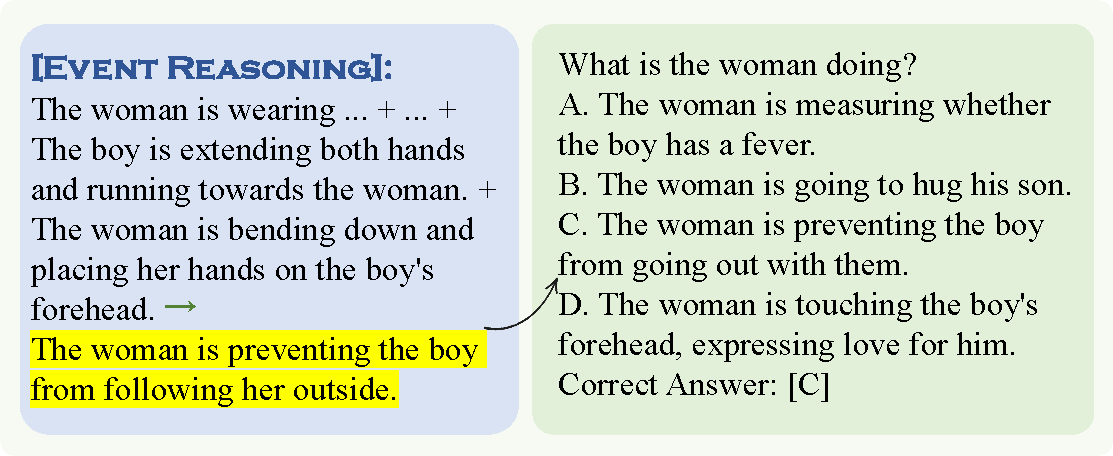
\includegraphics[width=0.45\textwidth]{figs/vqa_task_4.pdf}
  \caption{Generating a MCQ from event reasoning annotations.}
  \label{fig:qa_example}
\end{figure}
% \end{wrapfigure}

% The main idea of the question generation is that for each CoR, we can ask questions about both the conclusion (right part of $\rightarrow$) and reasons to draw the conclusion (left part of $\rightarrow$), as shown in Figure \ref{fig:qa_example}. 
% The process can be divided into two stages.
% \MY{The question generation strategy involves querying both the conclusion (right side of$\rightarrow$) and the reasoning behind it (left side of $\rightarrow$) for each CoR, as depicted in Figure \ref{fig:qa_example}.}

% \KZ{Reading this I still don't know how you do it with GPT. Does the prompt ask GPT to generate both the questions and answer options? How
% do you make sure the options include the correct answer, and where to to place the correct answer among the 4 positions?}

We use GPT-4 \cite{openai2023gpt4} to assist in generating the questions based on the annotation from Section \ref{sec:annotation}. % of each image. 
With annotated CoRs, both the conclusion (right side of$\rightarrow$) and the reasoning behind it (left side of $\rightarrow$) in each CoR can be used to generate questions and corresponding options, as depicted in Figure \ref{fig:qa_example}.
% The corresponding part in CoR is the correct option for each question.
These components in each CoR provide the correct options directly to the questions generated based on them. 
Specifically, this process is two-fold. 
1) \textbf{Automated Question Generation}: We use GPT-4 to generate questions for CogBench images, tailoring prompts for each reasoning category to produce CoR-related questions. The key point is to prompt GPT-4 to generate higher-quality distractors. An example prompt for this CoR-based GPT-assisted Question Generation approach is provided in Appendix B. %  \ref{sec:qa_prompt}
2) \textbf{Manual Refinement}: Despite GPT-4's capabilities, not all generated questions are optimal. In this stage, we manually refine the questions, ensuring they do not overtly favor the correct answer and that distractors are closely related to the question and misleading. 
Additionally, ChatGPT aids in identifying and filtering out simple questions that can be answered without image input.


% In the first stage, we use GPT-4 \cite{openai2023gpt4} to generate questions for images in CogBench. 
% For each category of reasoning capability, we design a sepcific prompt for GPT-4 to generate questions, so that questions related to different types of CoRs can be generated.
% For Question Generation, the key point is to generate high quality distractors. 
% Thus, we encourage GPT-4 to hallucinate to generate more perplexing distractors in our prompt. 
% Appendix \ref{sec:qa_prompt} shows an example of prompt we use for GPT-4 to generate questions.

% Though GPT-4 is powerful, it is still difficult for it to generate 100\% satisfying questions for all images.
% Thus, in the second stage, we manually select and modify the questions generated by GPT-4.
% The principle of selection and modification is that the question cannot apparently point to the correct option and distractors should be as closely related to the question and the correct option as possible, thereby possessing a certain level of misleadingness.
% During selection, ChatGPT is also utilized to help detect those simple questions that can be easily answered without having to accept the image as input. 



\subsection{CogBench Statistics}

\begin{table*}[th]
  \centering
  \small
  \setlength{\tabcolsep}{2.5pt} 

  \begin{tabular}{lcccccccc}
  \hline
  \textbf{} & \thead{\textbf{Time} } & \thead{\textbf{Location} } & \thead{\textbf{Character} } &  \thead{\textbf{Character}\\ \textbf{Relationship} } & \thead{\textbf{Event} } & \thead{\textbf{Event} \\ \textbf{Relationship} } & \thead{\textbf{Next Moment} \\ \textbf{Event} } & \thead{\textbf{Mental State} } \\ % \\ \textbf{Accuracy}
  \hline
  CoR & 47 & 179 & 106 & 263 &  701 & 425  & 107 & 417 \\
  QA & 86  & 220 & 162 & 317 & 658   &  402  & 135 & 597 \\  
  \hline
  \end{tabular}
  \caption{\label{tab:stat}
  Distribution of CoRs and questions in CogBench.
  }
\end{table*}

CogBench consists of 251 semantically-rich images with a total of 2670 entities, 2245 CoRs, 251 descriptions and 2577 questions, indicating the content contained in each image is complex, showcased in Table \ref{tab:stat}. 
% Figure \ref{fig:cogbench_stat} shows the distribution of these CoRs and questions.
%Table \ref{tab:stat} shows the distribution of these CoRs and questions.
% Though the number of images in CogBench is not large, 
% each image contains more CoRs and more questions can be asked.
The number of CoRs in event-related reasoning and [Mental State Reasoning] is large, which is a manifestation of the rich interesting stories in the images.
% indicating that images in CogBench contains a lot of interesting stories.
% \KZ{You didn't mention questions above? How did you get the questions?}

% % figure
% \begin{figure}[th]
%   \centering
%   % 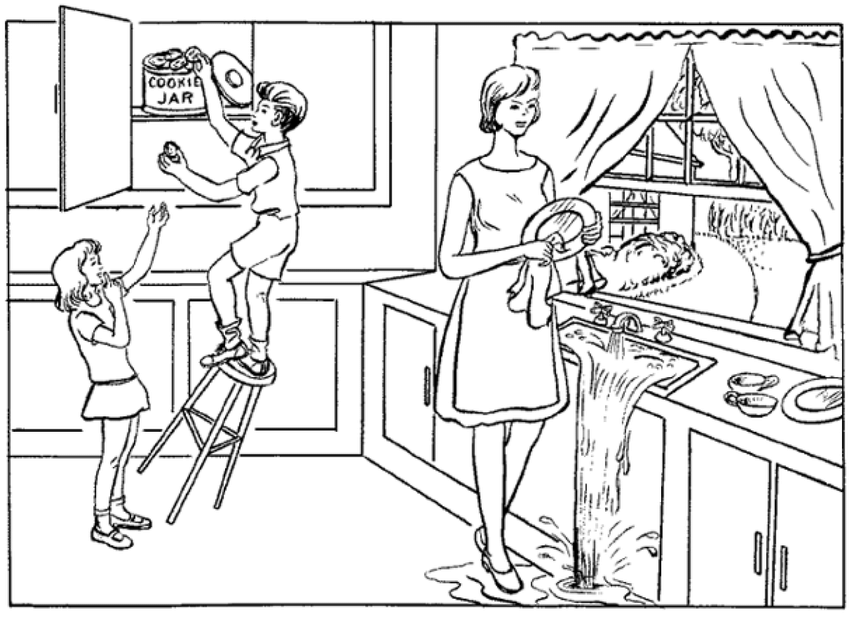
\includegraphics[width=0.4\textwidth]{figs/cookie_theft.png}
%   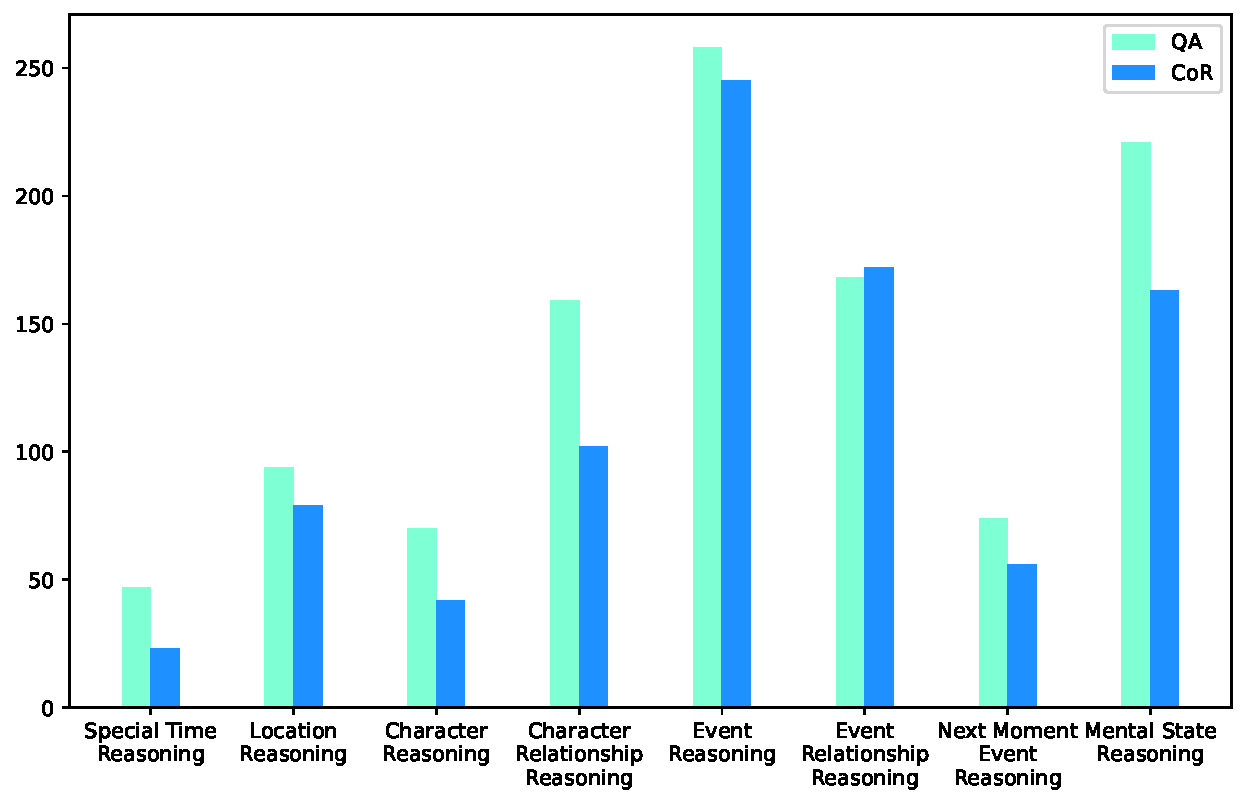
\includegraphics[width=0.48\textwidth]{figs/cogbench_stat.pdf}
%   \caption{Distribution of CoRs and questions in CogBench. \KZ{Fonts are
% too small. I repeat: text in figures and tables must be at least 2/3 of
% the size of main text.} \MY{Tables might be more suitable to show this stat. }}
%   % \footnote{https://dementia.talkbank.org/}
%   \label{fig:cogbench_stat}
% \end{figure}



